\section{Physical Network Service Composition}
Before venturing into Virtualized Network Functions, it needs to be clarified what network functions are in general, how they are implemented and composed \textit{physically}, and what the motivations are to move towards virtualizing them. 

Networks are the backbone of any modern IT infrastructure, and with the unstoppable rise of  Cloud Computing services their importance is ever increasing. This sharp rise in relevance causes the setup and operation of previously unthinkable data centers. Providing specific functioniality in such an environment has traditionally been the task of dedicated hardware that implemented services of many different domains. These include security functions that setup firewalls, scan for viruses and detect intruders but might be applied to ``...to any data plane packet processing and control plane function...''\cite{nfv_wp}. The advantage of using ASICs (Application-specific integrated circuit) lies in the potential for optimization. When designing a device that serves a very specific purpose, the application scenario can be anticipated much better than with general-purpose hardware. This typically leads to lower power consumption, higher efficiency and better output, but drives up the purchasing cost. Additionally, the operational cost is also high, since acquiring, configuring, deploying and maintaining such middleboxes is often a tedious, manual-heavy task. 

\begin{figure}[H]
	\centering
	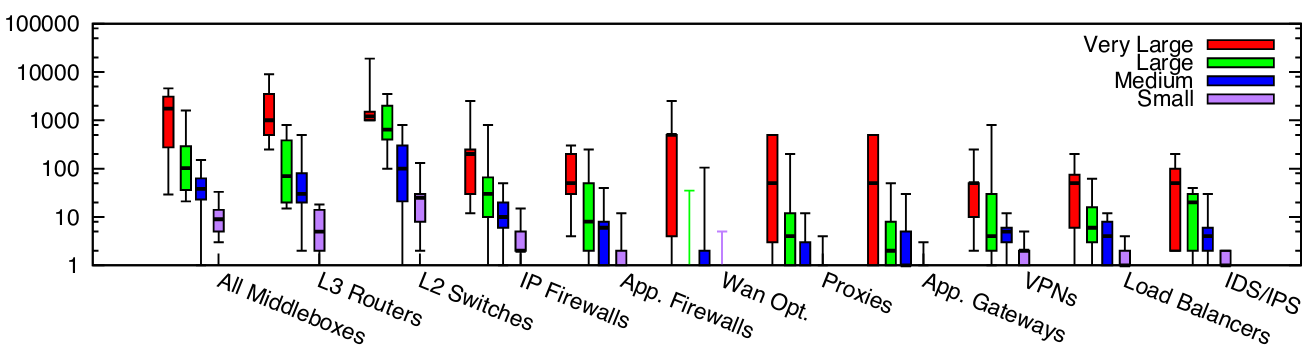
\includegraphics[width=1\linewidth]{images/middleboxesNumbers.png}
	\caption{Middlebox deployments in enterprise networks of various size (< 1k - >100k hosts). Y-axis in log scale, source \cite{sherry2016middleboxes}}
	\label{img:middleboxesNumbers}
\end{figure}

\begin{figure}[H]
	\centering
	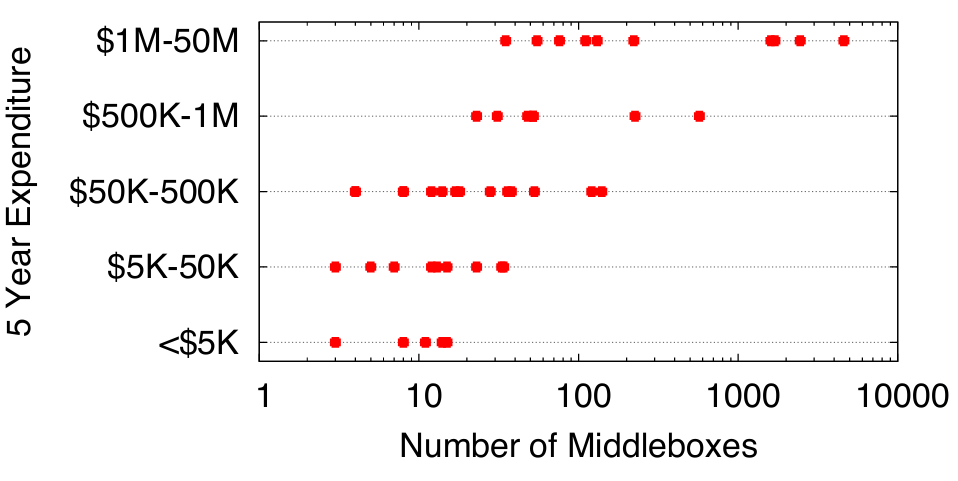
\includegraphics[width=1\linewidth]{images/middleboxesCost.png}
	\caption{Administrator-estimated spending on middlebox hardware per network \cite{sherry2016middleboxes}}
	\label{img:middleboxesCost}
\end{figure}

Figure \ref{img:middleboxesNumbers} illustrates the sheer amount of devices that are needed to guarantee the operation of enterprise networks of various size. Sherry \cite{sherry2012survey} \cite{sherry2016middleboxes} investigated their distribution among 57 educational and enterprise networks by surveying the operators for their experiences with the network appliances. Special focus was put on the quantity, their concerns, the cost and the ease of management. The results of this work give a good indication why this situation is unsustainable for future networks:  The number of these boxes is very high. To put it into perspective, the amount of these function specific devices approaches that of fundamental hardware like L3/L2 infrastructure. The associated cost of deploying such a large number of devices can be inspected in figure \ref{img:middleboxesCost} and indicates that investment cost is skyrocketing. Naturally, this might not be a problem for small companies that use a little amount of these devices. However, Cloud and Internet Service Providers rely on building, maintaining and reorganizing enormous computer networks and thus are driving forces behind alternative concepts in this domain \cite{sherry2016middleboxes} \cite{sherry2012survey}.

This will only gain importance with higher complexity and higher demand of the networks that are being built. Growing cloud data centers, implementation of 5G, further demanding services provided in the cloud like for instance Google Stadia, a streaming service for gaming. The last one is a very interesting scenario since low latency and high bandwidth is of utmost importance and needs to be guaranteed. Additionally, the provisioning and deployment of resources needs to happen instantly. This project might be paving the way for more ``serious'' applications like taking over functionality in autonomous driving. Fulfilling the such demanding requirements is only possible if the supporting network is highly flexible and can guarantee not only continuous connectivity, but also high performance. 

\section{Network Virtualization}
The previously described problem can only be solved when the need for the manual configuration and deployment that takes place on a box-to-box basis of function-specific hardware can be eliminated. The answer to this challenge is virtualization of the functionality in question which makes it both more configurable and highly maintainable. In order to take advantage of this virtualization, though, the encompassing network needs to support feasible possibilities to manage the virtual instances of network functions. Without a degree of automation and a centralized, programmatic approach, there would not be a huge benefit of going from physical to virtual. Software Defined Networking is ideal and often goes hand in hand with using these cutting edge technologies.

 Aside from the performance standpoint, this is also an ideal way to reduce cost significantly. This is due to multiple factors, such as the high purchasing cost of the middleboxes. Additionally, the devices often provide vendor-specific means for configuration which entails high administrative and operational cost since personnel training and special spare parts are needed.  The investment into retraining the staff that has to work with such devices can even influence the decision making process since without the expertise, smooth operations of the network are questionable. 

Once it is time to update or upgrade the parts of the network that provide certain functionality, another downside becomes quickly apparent: the only way to to get the newest features is to replace the outdated hardware with the newer model. And if more instances of the functionality is needed, there acquiring more devices is the only choice to allow for scalability or provide fault tolerance via replication. 

As already mentioned, virtualization and providing the network functionality as software packages that can run on general-purpose hardware anywhere is the core promise of network virtualization. This paradigm has caused a paradigm shift in recent years in networking that has lead to many projects and software solutions. In the following sections Software Defined Networking (SDN), Network Function Virtualization and Virtualized Network Functions will be briefly introduced as the main driving forces and central ideas behind the virtualization efforts. 


\subsection{Software Defined Networking}
\label{sec:sdn}

The unobstructed operation of highly distributed applications and the offer of services depends highly on mitigating faults in the network and the appropriate reaction to fluctuating load. In traditional networks, there is hardly any support to implement automatic policy change as a reaction to events like spikes in load or the reconfiguration when faults occur in the system \cite{kreutz2015software}. When faced with such situations, ''[\dots] every single hardware instance [\dots]`` \cite{grossmann2013auto} is in need for manipulation to realize the desired change.  The need for manual intervention is responsible for immense risk \todo{GO ON HERE}

The concept of Software Defined Networking focuses on allowing for a (re-)configuration effort that works through software and eliminates the need for repetitive, vendor-specific and manual setup and administrative tasks.  

\begin{comment}
	
The resulting complexity renders such networks almost static, since the maintenance, the update effort and associated risk of service disruption is skyrocketing. This process of slowing down innovation, the evolution of the Internet and network technology is often described by the term \textit{ossification} \cite{nunes2014survey}. 

\hyphenation{par-a-digm}
As a reaction to the growing inadequateness of traditional networks, the architectural paradigm of Software-defined Networking has gained a lot of momentum and popularity. One of the core principles that enables higher flexibility is the separation of the control plane from the data plane. Networking hardware has long been \textit{vertically integrated}, meaning that these two planes had been both represented in the device itself, isolating it from external manipulation and "[...] reducing flexibility and hindering innovation [...]" \cite{kreutz2015software}. The resulting control layer abstracts from all network devices that formerly were tightly coupled, thus abolishing the need for manual and individual configuration. A comparison between these two concepts can be seen in figure \ref{img:sdn}. 


\begin{figure}[H]
	\centering
	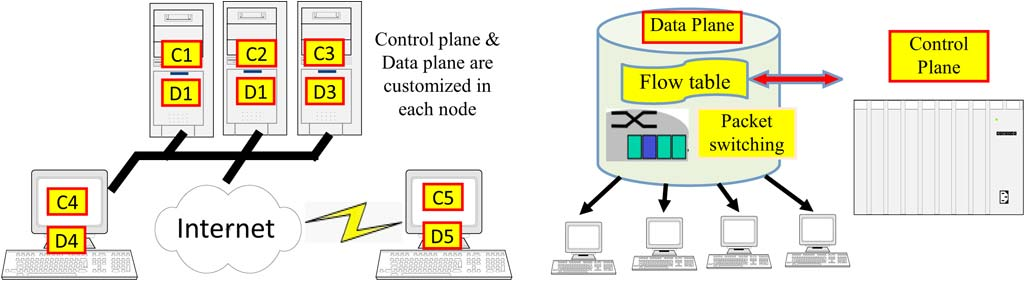
\includegraphics[width=1\textwidth]{images/sdn.png}
	\caption{Comparison between traditional (left) and Software-defined Networks (right), source \cite{hu2014survey}}
	\label{img:sdn}
\end{figure}

On the left, the control and the data plane are vertically integrated in each device, whereas on the right, the devices are only concerned with forwarding traffic and the control part is extracted into a separate layer. SDN controllers located on this layer can offer a logically centralized access to manage and program connected switches, routers and other middleboxes via a common protocol. This decoupling considerably reduces the effort that has to be put in when a change in the network structure or policy is desired. To add, many SDN controllers support the integration of custom applications, which enable the tailoring of the controller to the needs of a specific network without having to wait for a particular vendor to integrate the requested feature. 

The programming of the network hardware is realized by using a standardized protocol for communication, depending on what the controller and the managed switches require. One protocol used for this purpose is OpenFlow. The application programming interface (API) that connects the controller to the network infrastructure via this protocol is called the Southbound API as can be seen in figure \ref{img:sdnAPIs}, where the middle box contains the SDN controller software.
Situated to the left, multiple instances of the controller can communicate with each other. This so-called westbound API allows for the distribution of the network management duties among more than one controller. This helps guarantee higher availability, fault tolerance and scalability. Additionally, separation of concerns can be realized by letting specific instances take care of one logically coherent part of network infrastructure and its devices. To the right side the eastbound API allows for the communication with traditional, non-SDN networks which provides downward compatibility. The implementation is highly dependent on the protocols and technology employed in the legacy networks. 

\begin{figure}[H]
	\centering
	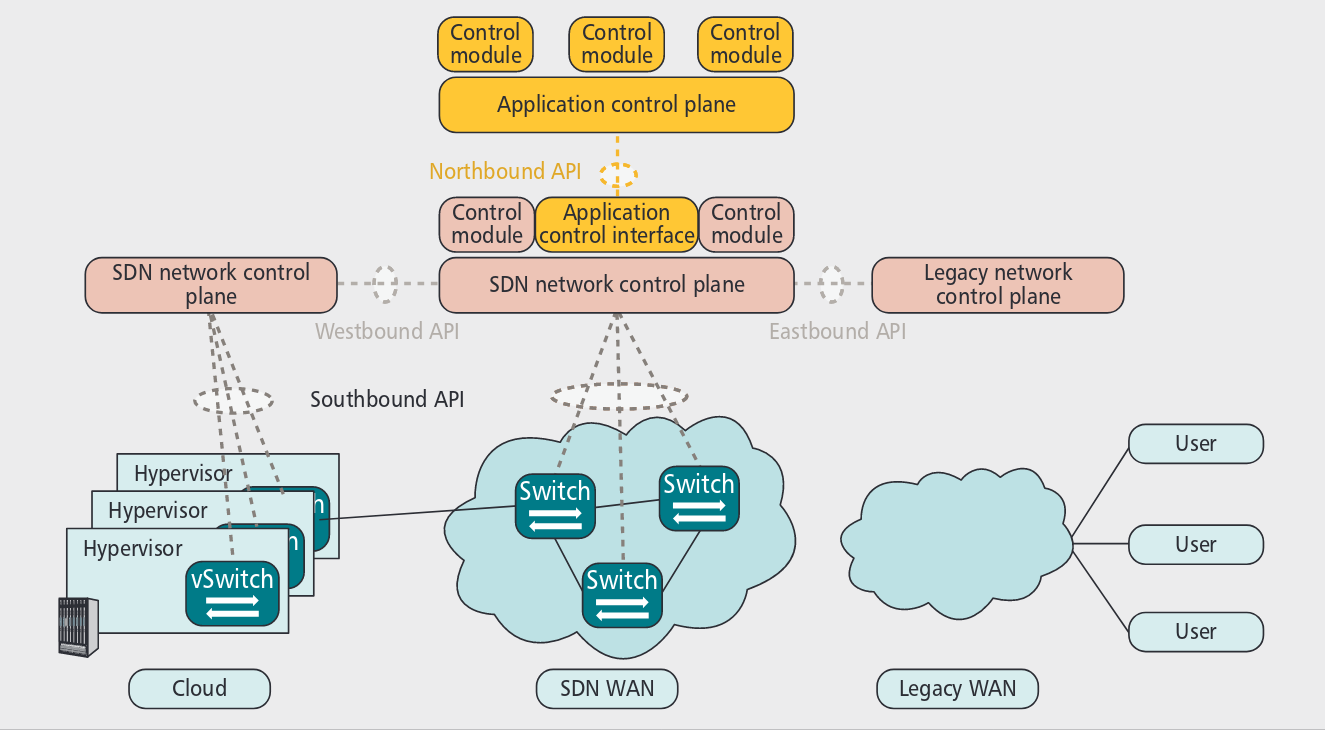
\includegraphics[width=1\textwidth]{images/sdnAPIs.png}
	\caption{The different elements of the SDN architecture, connected via APIs, source \cite{jarschel2014interfaces}}
	\label{img:sdnAPIs}
\end{figure}

This distinction between east and westbound is not present in all architecture specifications and omitted in Sezer \textit{et al.} \cite{sezer2013we} for instance. In this approach both the east and the westbound APIs serve the inter cluster communication of multiple controller instances. Finally, the diagram also expands towards the top via the Northbound API connecting an application context to the SDN controller. This illustrates the possibility of expansion by implementing custom apps that can access the core services provided by the SDN controller  \cite{hu2014survey} \cite{jarschel2014interfaces} \cite{nunes2014survey} \cite{sezer2013we} \cite{shin2012software} \cite{jammal2014software}.

\end{comment}


\subsection{VNF}

\subsection{NFV and NFVI}

Network 

\begin{figure}[H]
	\centering
	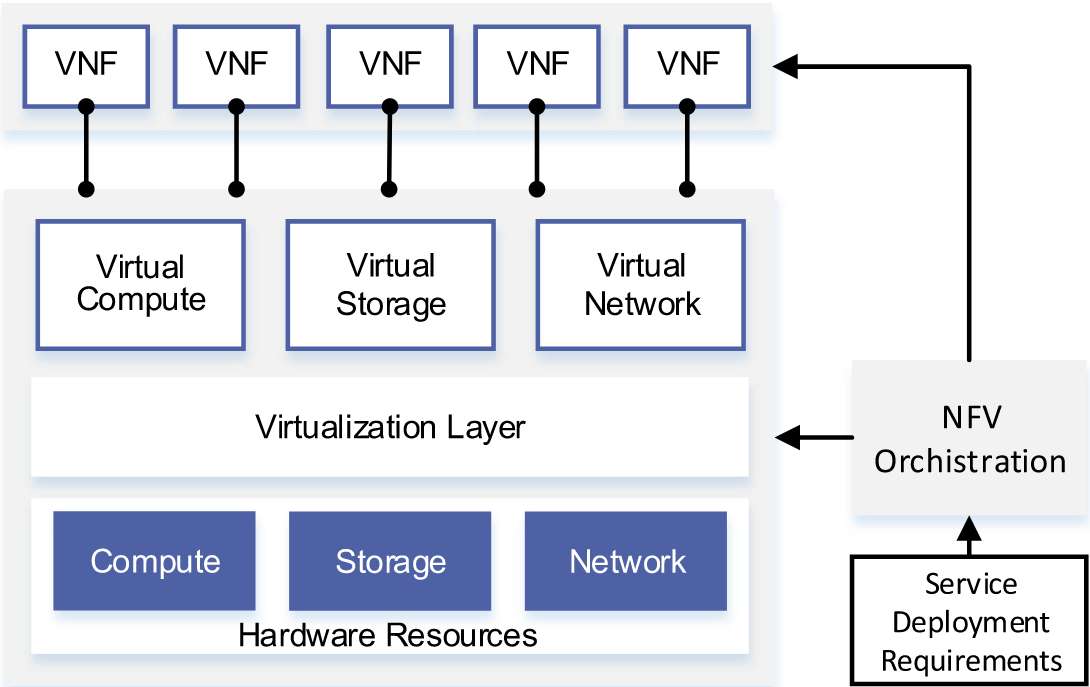
\includegraphics[width=1\linewidth]{images/nfvi.png}
	\caption{This is the caption \cite{li2015software}}
	\label{img:nfvi}
\end{figure}

\subsection{SDN and NFV}

\begin{comment}
	
In addition to the purchasing cost, the boxes have to be installed and maintained, causing administrative and operative cost. Since the nature of such devices is proprietary on a hard- and software level, training of personnel has to take vendor specific configuration into consideration. This can even influence the decision whether to invest in a specific implementation of middleboxes, since without the required expertise, the products could seriously endanger any potential profit. 

Scalability and fault tolerance are often enhanced by introducing additional and redundant devices into the network, adding to the operational cost. Finally, once newer functionality is released on the market, old middleboxes have no possibility of being upgraded. The only way of making use of up-to-date features is to replace the hardware in question \cite{wood2015toward} \cite{sherry2012survey} \cite{bari2015orchestrating} \cite{mekky2017network}.

Turning away from application-specific integrated circuits towards software-based solutions that can be run on general-purpose hardware is the core proposal of Network Function Virtualization. The concept of NFV has been proposed by a special interest group that is part of the European Telecommunications Standards Institute (ETSI) in a white paper in 2012 \cite{nfvWhitePaper}. Since then, the proposal has gained a lot of momentum and is taken into consideration when planing the networks of the future \cite{ordonez2017network}.

\begin{figure}[H]
	\centering
	%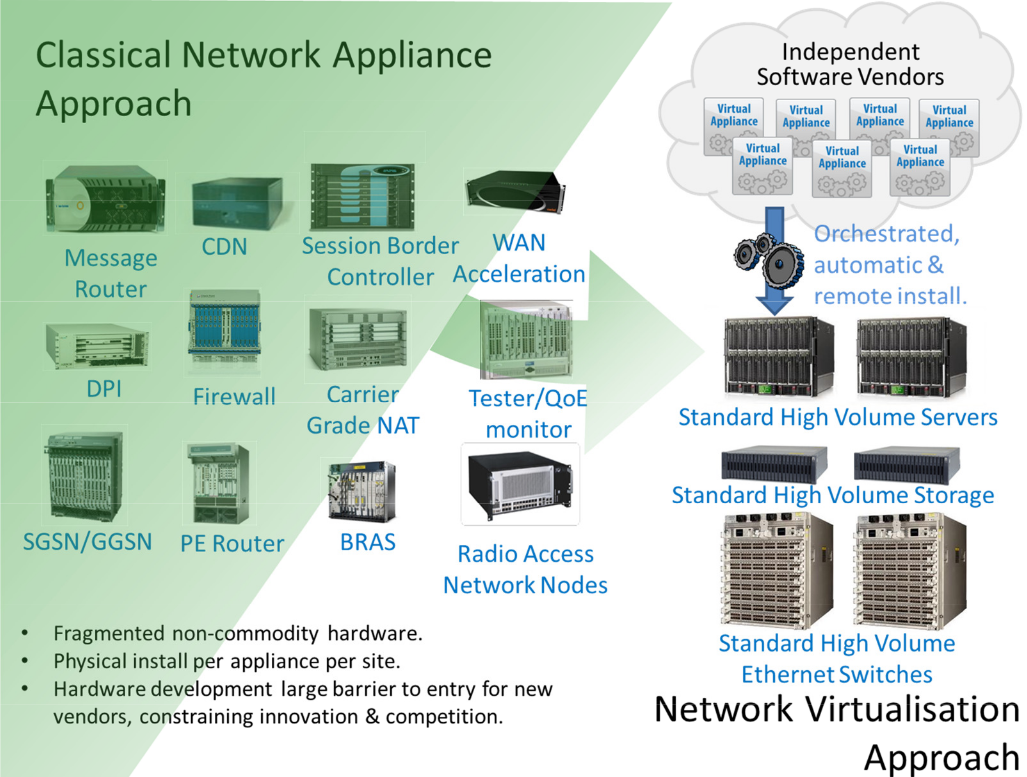
\includegraphics[width=0.85\textwidth]{images/nfv.png}
	\caption{From ASICs, to virtual appliances, source \cite{nfvWhitePaper}}
	\label{img:nfv}
\end{figure}
The core vision, as taken from the introductory white paper, is to break up the tight coupling of function and physical appliance. Figure \ref{img:nfv} shows this transition from several, tightly and vertically integrated hardware middleboxes, towards a system where the desired services are provided in virtual form by independent software vendors (top right). The underlying hardware consists of devices that can already be found in data centers, like standard high volume servers, storage and Ethernet switches. The deployment of the virtual appliances no longer requires tedious, manual and a per device setup and configuration but can rather be done in an orchestrated, automatic and remote way. The definition of such services has now also been decoupled from hardware development, favoring the emergence of a broader software ecosystem. In this environment the supply of possible network functions rises and updated or new functionality can be obtained remotely. This concept benefits highly from being used in a network environment that realizes SDN principles. The whitepaper, laying out the core principles, even includes a passage that specifies the relationship between NFV and SDN as mutually beneficial: "[...] SDN can enhance performance, simplify compatibility with existing deployments, and facilitate operation and maintenance procedures", while NFV "[...] is able to support SDN by providing the infrastructure upon which the SDN software can be run"\cite{nfvWhitePaper}. 

\end{comment}
